\documentclass{beamer}

\usepackage{amsmath}
\usepackage{tikz}

\graphicspath{{figures/}}
\DeclareGraphicsExtensions{.pdf,.png,.jpg}

\usetikzlibrary{arrows,shapes}

\title[Quantum GI]
{Distinguishing graphs with a quantum annealer
  using susceptibility measurements} 

\author[Wittmann, Hen, Young]
{Matthew~Wittmann\inst{1} \and Itay~Hen\inst{2} \and A.~P.~Young\inst{1}}

\institute[UCSC and ISI]
{
  \inst{1}%
  Physics Department\\
  University of California, Santa Cruz
  \and
  \inst{2}%
  Information Sciences Institute\\
  University of Southern California
}
\date[APS MM 2014]{APS March Meeting, 2014}

\begin{document}

% TikZ commands needed for fancy equation annotation
% see http://www.texample.net/tikz/examples/beamer-arrows/
\tikzstyle{every picture}+=[remember picture]
\tikzstyle{na} = [baseline=-.5ex]
\everymath{\displaystyle}

\frame{\titlepage}
\section{Background}
\begin{frame}
  \frametitle{Introduction}
\end{frame}
\begin{frame}
  \frametitle{Graph Isomorphism (GI) Problem}
  Given two graphs, determine whether one can be obtained from the other by
  relabeling the vertices. If so, the graphs are \alert{isomorphic}.
  \begin{columns}[t]
    \column{0.25\textwidth}
    \begin{block}{$G=(E_G,\,V_G)$}
      \begin{minipage}[t][0.45\textheight][c]{\textwidth}
        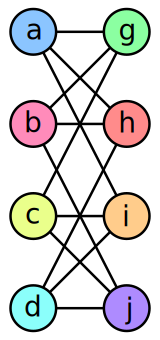
\includegraphics[scale=0.4]{Graph_isomorphism_a}
      \end{minipage}
    \end{block}
    \column{0.25\textwidth}
    \begin{block}{$H=(E_H,\,V_H)$}
      \begin{minipage}[t][0.45\textheight][c]{\textwidth}
        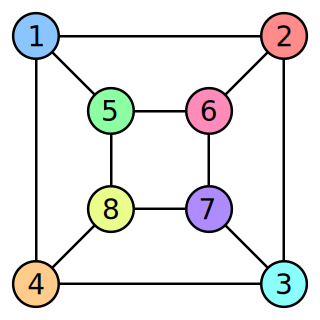
\includegraphics[scale=0.4]{Graph_isomorphism_b}
      \end{minipage}
    \end{block}
    \column{0.25\textwidth}
    \abovedisplayskip=0pt
    \abovedisplayshortskip=0pt
    \begin{block}{$f: V_G\rightarrow V_H$}
      \begin{align*}
        f(a) &= 1 \\
        f(b) &= 6 \\
        f(c) &= 8 \\
        f(d) &= 3 \\
        f(g) &= 5 \\
        f(h) &= 2 \\
        f(i) &= 4 \\
        f(j) &= 7
      \end{align*}
    \end{block}
  \end{columns}
\end{frame}
\begin{frame}
  \frametitle{Properties of the GI Problem}
  \begin{itemize}
    \item Complexity class \alert{NP}, but unlikely to be NP-complete
  \end{itemize}
\end{frame}
\begin{frame}
  \frametitle{Co-Ising graphs}
  Encode graph $G=(V,\,E)$ as an Ising Hamiltonian $H(G)$
  \begin{itemize}
    \item 1-1 mapping of vertices to Ising spins
    \item<2-> \alert{Antiferromagnetic} interaction between spins $\sigma_i$
      and $\sigma_j$ for each edge $(i,\,j) \in E$
      \tikz[na]\node [coordinate] (n1) {};
  \end{itemize}
  \begin{equation*}
    \onslide<2->{ % only show AFM term starting on slide 2
      H(G) = 
      \tikz[baseline]{
        \node[fill=blue!20,ellipse,anchor=base] (t1)
        {$\sum_{(i,\,j) \in E} \sigma^z_i \sigma^z_j$};
      }
    }
    \onslide<3->{ % only show field term starting on slide 3
      -
      \tikz[baseline]{
        \node[fill=red!20,ellipse,anchor=base] (t2)
        {$h \sum \sigma^z_i$};
      }
    }
  \end{equation*}
  \begin{itemize}
    \item<3-> \alert{Longitudinal field} to break symmetry
      \tikz[na]\node [coordinate] (n2) {};
  \end{itemize}

  % Draw edges from bullet points to terms (note 'overlay' style).
  \begin{tikzpicture}[overlay]
    \path[->]<2-> (n1) edge [out=0,in=90] (t1);
    \path[->]<3-> (n2) edge [out=0,in=-90] (t2);
  \end{tikzpicture}
  \begin{definition}<4>
    $G_1,\,G_2$ \alert{co-Ising} $\iff$ $H(G_1)$, $H(G_2)$ co-spectral for all $h$
  \end{definition}
\end{frame}
\begin{frame}
  \frametitle{Method}
  \begin{equation*}
    H(G) = s H_p(G) + (1-s) \sum \sigma^x_i
  \end{equation*}
\end{frame}
\begin{frame}
  \frametitle{Results}
\end{frame}
\end{document}
